\documentclass[presentation]{beamer}

\usepackage[utf8]{inputenc}
% \usepackage[T1]{fontenc}
\usepackage{fixltx2e}
\usepackage{graphicx}
% \usepackage{longtable}
% \usepackage{tabu}
\usepackage{makecell}
\usepackage{float}
\usepackage{subcaption}
\usepackage{wrapfig}
\usepackage{rotating}
\usepackage[normalem]{ulem}
\usepackage{amsmath}
% \usepackage{textcomp}
% \usepackage{marvosym}
% \usepackage{wasysym}
% \usepackage{amssymb}
\usepackage{hyperref}
\usepackage{ragged2e}
\usepackage{xcolor}


\usepackage{bm}

\usepackage{amsmath,amssymb}
\newcommand{\bx}{\mathbf{x}}
\newcommand{\bv}{\mathbf{v}}
\newcommand{\bp}{\mathbf{p}}
\newcommand{\bq}{\mathbf{q}}
\newcommand{\by}{\mathbf{y}}

\newcommand{\bbR}{\mathbb{R}}
\newcommand{\bbN}{\mathbb{N}}

\newcommand{\bxi}{\bm{\xi}}
\newcommand{\bal}{\bm{\alpha}}
\newcommand{\bth}{\bm{\theta}}

\usepackage{etoolbox}
\let\bbordermatrix\bordermatrix
\patchcmd{\bbordermatrix}{8.75}{4.75}{}{}
\patchcmd{\bbordermatrix}{\left(}{\left[}{}{}
\patchcmd{\bbordermatrix}{\right)}{\right]}{}{}

\usepackage[authoryear, round]{natbib}

\newcommand{\sidebysidecaption}[4]{%
\RaggedRight%
  \begin{minipage}[t]{#1}
    \vspace*{0pt}
    #3
  \end{minipage}
  \hfill%
  \begin{minipage}[t]{#2}
    \vspace*{0pt}
    #4
\end{minipage}%
}

%% colors
\definecolor{Red}{rgb}{0.7,0,0}
\definecolor{Blue}{rgb}{0,0,0.8}
\definecolor{Green}{rgb}{0,0.8,0}
\definecolor{Gray}{rgb}{0.8,0.8,0.8}
\definecolor{Orange}{rgb}{1,.65,0}

\usepackage{hyperref}
\hypersetup{
  hyperindex = {true},
  colorlinks = {true},
  linktocpage = {true},
  plainpages = {false},
  linkcolor = {Blue},
  citecolor = {Blue},
  urlcolor = {Red},
  pdfstartview = {Fit},
  pdfpagemode = {UseOutlines},
  pdfview = {XYZ null null null},
  pdfkeywords={proteomics, spatial, dynamics, integration, regulation, computational biology},
  pdfsubject={Research talk},
  pdfcreator={Laurent Gatto}}

%% knitr

%% maxwidth is the original width if it is less than linewidth
%% otherwise use linewidth (to make sure the graphics do not exceed the margin)
\makeatletter
\def\maxwidth{ %
  \ifdim\Gin@nat@width>\linewidth
    \linewidth
  \else
    \Gin@nat@width
  \fi
}
\makeatother

\definecolor{fgcolor}{rgb}{0.345, 0.345, 0.345}
\newcommand{\hlnum}[1]{\textcolor[rgb]{0.686,0.059,0.569}{#1}}%
\newcommand{\hlstr}[1]{\textcolor[rgb]{0.192,0.494,0.8}{#1}}%
\newcommand{\hlcom}[1]{\textcolor[rgb]{0.678,0.584,0.686}{\textit{#1}}}%
\newcommand{\hlopt}[1]{\textcolor[rgb]{0,0,0}{#1}}%
\newcommand{\hlstd}[1]{\textcolor[rgb]{0.345,0.345,0.345}{#1}}%
\newcommand{\hlkwa}[1]{\textcolor[rgb]{0.161,0.373,0.58}{\textbf{#1}}}%
\newcommand{\hlkwb}[1]{\textcolor[rgb]{0.69,0.353,0.396}{#1}}%
\newcommand{\hlkwc}[1]{\textcolor[rgb]{0.333,0.667,0.333}{#1}}%
\newcommand{\hlkwd}[1]{\textcolor[rgb]{0.737,0.353,0.396}{\textbf{#1}}}%

\usepackage{framed}
\makeatletter
\newenvironment{kframe}{%
 \def\at@end@of@kframe{}%
 \ifinner\ifhmode%
  \def\at@end@of@kframe{\end{minipage}}%
  \begin{minipage}{\columnwidth}%
 \fi\fi%
 \def\FrameCommand##1{\hskip\@totalleftmargin \hskip-\fboxsep
 \colorbox{shadecolor}{##1}\hskip-\fboxsep
     % There is no \\@totalrightmargin, so:
     \hskip-\linewidth \hskip-\@totalleftmargin \hskip\columnwidth}%
 \MakeFramed {\advance\hsize-\width
   \@totalleftmargin\z@ \linewidth\hsize
   \@setminipage}}%
 {\par\unskip\endMakeFramed%
 \at@end@of@kframe}
\makeatother

\definecolor{shadecolor}{rgb}{.97, .97, .97}
\definecolor{messagecolor}{rgb}{0, 0, 0}
\definecolor{warningcolor}{rgb}{1, 0, 1}

\definecolor{errorcolor}{rgb}{1, 0, 0}
\newenvironment{knitrout}{}{} % an empty environment to be redefined in TeX

\usepackage{alltt}
\usepackage[utf8]{inputenc}
\usepackage[T1]{fontenc}
\usepackage{fixltx2e}
\usepackage{graphicx}
\usepackage{longtable}
\usepackage{float}
\usepackage{wrapfig}
\usepackage{rotating}
\usepackage[normalem]{ulem}
\usepackage{amsmath}
\usepackage{textcomp}
\usepackage{marvosym}
\usepackage{wasysym}
\usepackage{amssymb}


\date{30 November 2018\\ Interuniversity Institute of Bioinformatics in Brussels}

\title{Probabilistic modelling of protein sub-cellular localisation}

\author{Laurent Gatto\\
  \url{laurent.gatto@uclouvain.be}\\
  de Duve Institute -- \textbf{UCLouvain}
}


% \AtBeginSection[] % Do nothing for \section*
% {
%   \begin{frame}<beamer>
%     \frametitle{Plan}
%     \tableofcontents[currentsection]
%   \end{frame}
% }


\begin{document}

\maketitle

% \begin{frame}{}
%   Who?
% \end{frame}

\begin{frame}{Abstract}
  Computational sciences can be and extremely valuable, or arguably
  essential, when exploring large and complex bio-medical data. In my
  presentation, I will illustrate this claim using examples from my
  work on protein sub-cellular localisation using mass spectrometry. I
  will present some computational discoveries and developments that
  helped putting protein sub-cellular localisation experiments under a
  new light, and illustrate the evolution and challenges of some of
  these developments.
\end{frame}

\begin{frame}
  \begin{block}{}
  \begin{enumerate}
  \item \textbf{Use case}: spatial proteomics.
  \item Novel \textbf{computational biology research and developments}
    to acquire reliable biological knowledge.
  \item \textbf{Behind the scenes}: software/data structures and open research
    practice.
  \end{enumerate}
  \end{block}
\end{frame}


\section{Spatial proteomics}

\begin{frame}{}
  \begin{center}
    \Large{\textbf{Use case}: spatial proteomics.}
  \end{center}
\end{frame}

\subsection*{The LOPIT pipeline}

\label{sec:spintro}

%% \begin{frame}{Regulations}
%%   \begin{figure}[h]
%%     \centering
%%     \includegraphics[width=1\linewidth]{Figures2/regulation.jpg}
%%   \end{figure}
%% \end{frame}

\label{sec:spspatprot}

\begin{frame}{Cell organisation - regulation of protein localisation}
  \begin{center}
    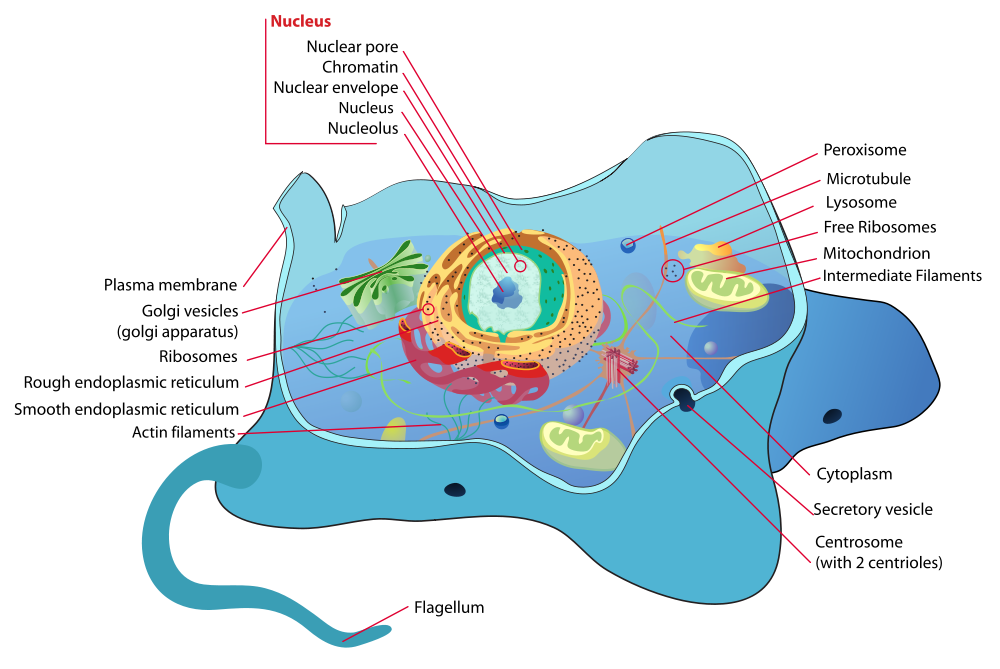
\includegraphics[width=1\linewidth]{Figures/Animal_cell_structure.png} \\
    \textbf{\textcolor{Blue}{Spatial proteomics}} is the systematic
    study of protein localisations.
  \end{center}

  \tiny Image from Wikipedia
  \url{http://en.wikipedia.org/wiki/Cell_(biology)}.
\end{frame}

% \begin{frame}{Spatial proteomics - Why?}
%   \begin{itemize}
%   \item Localisation is function
%   \item Mis-localisation \citep{Kau2004,Laurila2009}
%   \item Re-localisation
%   \end{itemize}
% \end{frame}

\begin{frame}{Spatial proteomics - Why?}
  \begin{block}{Localisation is function}
    \begin{itemize}
    \item The cellular sub-division allows cells to establish a range
      of distinct micro-environments, each favouring different
      biochemical reactions and interactions and, therefore, allowing
      each compartment to fulfil a particular functional role.
    \item Localisation and sequestration of proteins within
      sub-cellular niches is a fundamental mechanism for the
      post-translational regulation of protein function.
    \end{itemize}
  \end{block}
  \begin{block}{Re-localisation in}
    \begin{itemize}
    \item \textcolor{Blue}{Differentiation} stem cells.
    \item \textcolor{Blue}{Activation} of biological processes.
    \end{itemize}
    %% Examples later.
  \end{block}
\end{frame}

\begin{frame}{Spatial proteomics - Why?}
  \begin{block}{Mis-localisation}
    Disruption of the targeting/trafficking process alters proper
    sub-cellular localisation, which in turn perturb the cellular
    functions of the proteins.
    \begin{itemize}
    \item Abnormal protein localisation leading to the \textbf{loss of
        functional} effects in diseases \citep{Laurila2009}.
    \item Disruption of the nuclear/cytoplasmic transport (nuclear
      pores) have been detected in many types of \textbf{carcinoma
        cells} \citep{Kau2004}.
    \item Sub-cellular localisation of MC4R with ADCY3 at neuronal
      primary cilia underlies a common pathway for genetic
      predisposition to \textbf{obesity} \citep{Siljee:2018}.
    \end{itemize}
  \end{block}

\end{frame}


\subsubsection*{Experimental designs}
\label{sec:expdesign}

\begin{frame}{Spatial proteomics - How, experimentally}
  \begin{figure}
    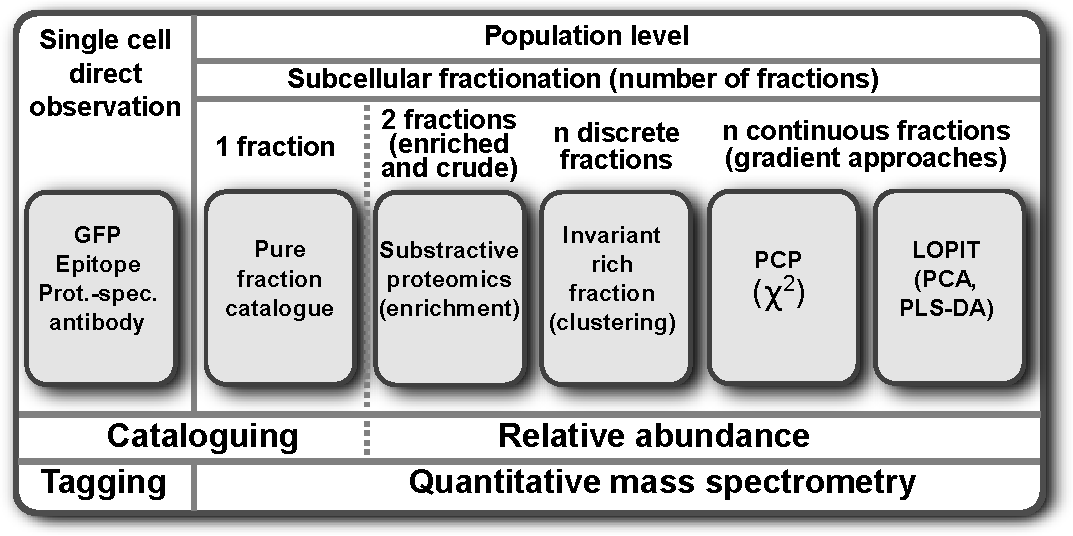
\includegraphics[width=.8\linewidth]{Figures/F02-expdesigns.pdf}
    \caption{Organelle proteomics approaches \citep{Gatto:2010}}
  \end{figure}
\end{frame}

\begin{frame}{Fusion proteins and immunofluorescence}

  \begin{figure}[h]
    \centering
    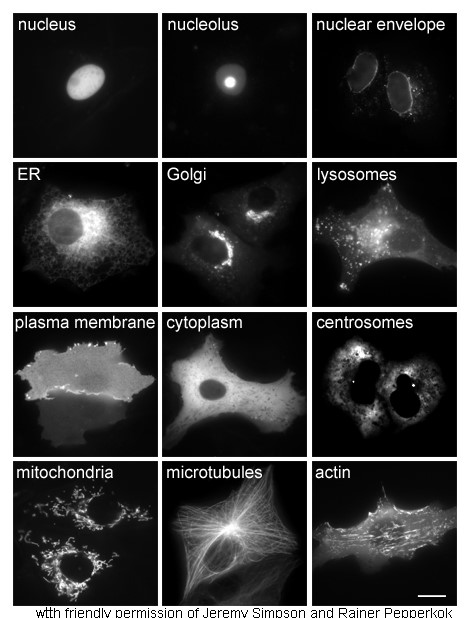
\includegraphics[width=.35\linewidth]{Figures2/Localisations02eng.jpg}
    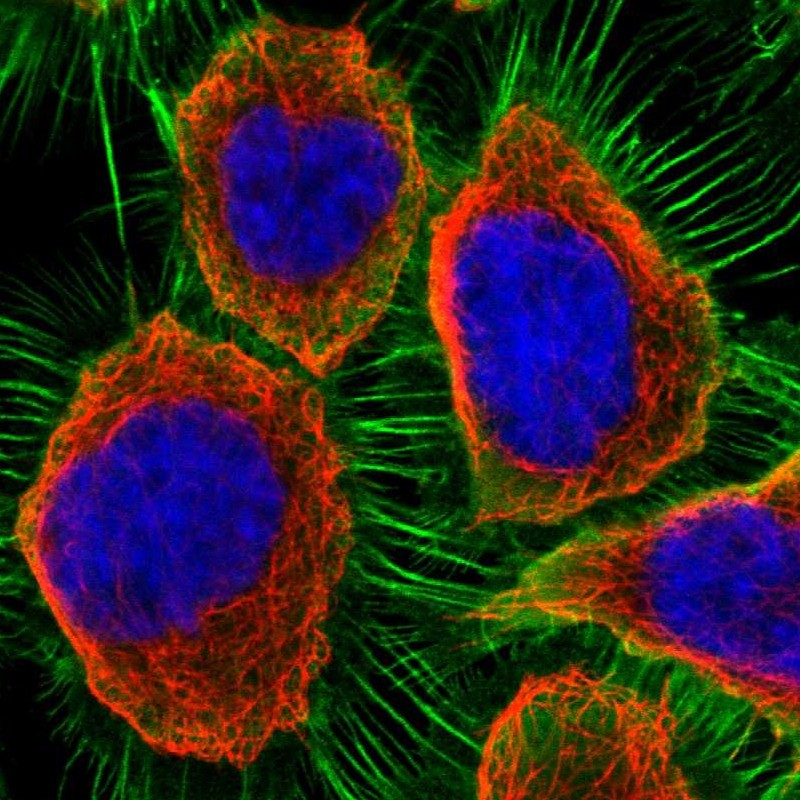
\includegraphics[width=.45\linewidth]{figures/if_selected.jpg}
    \caption{Targeted protein localisation. Example of discrepancies
      between IF and FPs as well as between FP tagging at the N and C
      termini \citep{Stadler:2013}.}
  \end{figure}
\end{frame}


\subsubsection*{Gradient approaches}
\label{sec:grad}

\begin{frame}{Spatial proteomics - How, experimentally}
  \begin{figure}
    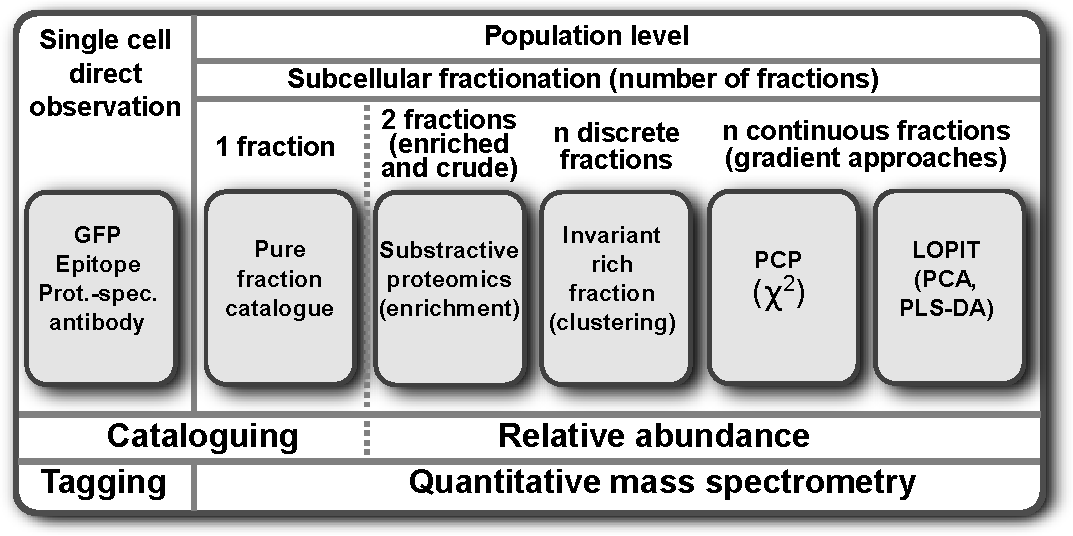
\includegraphics[width=.8\linewidth]{Figures/F02-expdesigns.pdf}
    \caption{Organelle proteomics approaches
      \citep{Gatto:2010}.}
  \end{figure}

  \textbf{Gradient approaches}: \cite{Dunkley:2006},
  \cite{Foster2006}.

  \bigskip

  \textbf{Explorative/discovery approaches},
  \textcolor{Blue}{steady-state \textbf{global localisation maps}}.
\end{frame}


\begin{frame}{}
  \begin{figure}
    % \includegraphics[width=.8\linewidth]{Figures/F03-protocols-8plex.pdf}
    % \includegraphics[width=.5\linewidth]{figures/expdesign.pdf}
    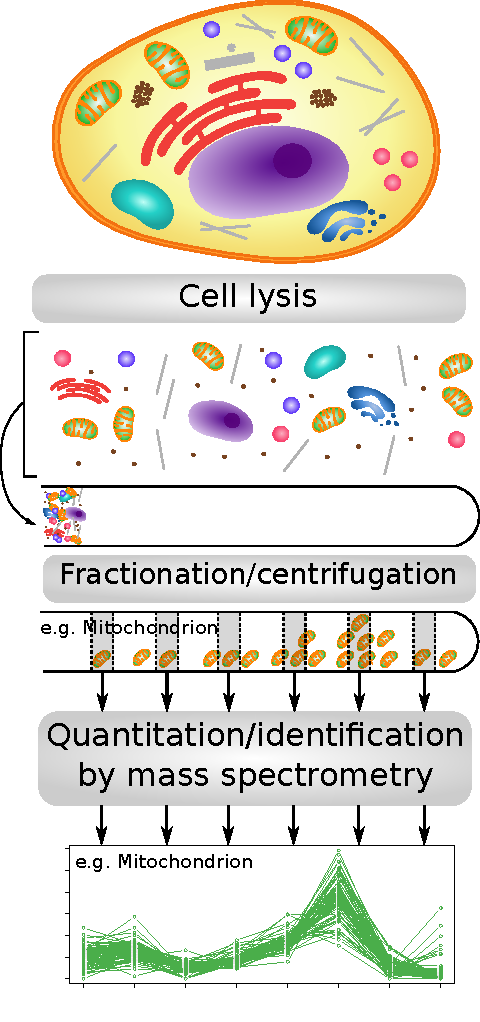
\includegraphics[width=.39\linewidth]{figures/workflow_primary.pdf}
  \end{figure}
\end{frame}

\subsubsection*{The data}
\label{sec:data}

\begin{frame}{Quantitation data}
  \begin{center}
    \begin{tabular}{|l|llll|}
      \hline
      & Fraction$_{\text{1}}$ & Fraction$_{\text{2}}$ & \ldots{} & Fraction$_{\text{m}}$ \\
      \hline
      p$_{\text{1}}$ & q$_{\text{1,1}}$ & q$_{\text{1,2}}$ & \ldots{} & q$_{\text{1,m}}$ \\
      p$_{\text{2}}$ & q$_{\text{2,1}}$ & q$_{\text{2,2}}$ & \ldots{} & q$_{\text{2,m}}$ \\
      p$_{\text{3}}$ & q$_{\text{3,1}}$ & q$_{\text{3,2}}$ & \ldots{} & q$_{\text{3,m}}$ \\
      p$_{\text{4}}$ & q$_{\text{4,1}}$ & q$_{\text{4,2}}$ & \ldots{} & q$_{\text{4,m}}$ \\
      \vdots & \vdots & \vdots & \vdots & \vdots \\
      p$_{\text{j}}$ & q$_{\text{j,1}}$ & q$_{\text{j,2}}$ & \ldots{} & q$_{\text{j, m}}$ \\
      \hline
    \end{tabular}
  \end{center}
\end{frame}

\begin{frame}{Quantitation data and organelle markers}
  \begin{center}
    \begin{tabular}{|l|llll||l|}
      \hline
      & Fraction$_{\text{1}}$ & Fraction$_{\text{2}}$ & \ldots{} & Fraction$_{\text{m}}$ & markers\\
      \hline
      p$_{\text{1}}$ & q$_{\text{1,1}}$ & q$_{\text{1,2}}$ & \ldots{} & q$_{\text{1,m}}$ & unknown \\
      p$_{\text{2}}$ & q$_{\text{2,1}}$ & q$_{\text{2,2}}$ & \ldots{} & q$_{\text{2,m}}$ & \textcolor{Red}{$loc_{1}$}\\
      p$_{\text{3}}$ & q$_{\text{3,1}}$ & q$_{\text{3,2}}$ & \ldots{} & q$_{\text{3,m}}$ & unknown \\
      p$_{\text{4}}$ & q$_{\text{4,1}}$ & q$_{\text{4,2}}$ & \ldots{} & q$_{\text{4,m}}$ & \textcolor{Blue}{$loc_{i}$}\\
      \vdots & \vdots & \vdots & \vdots & \vdots & \vdots\\
      p$_{\text{j}}$ & q$_{\text{j,1}}$ & q$_{\text{j,2}}$ & \ldots{} & q$_{\text{j, m}}$ & unknown \\
      \hline
    \end{tabular}
  \end{center}
\end{frame}


\section{Computational infrastructure}

\begin{frame}{}
  \begin{center}
    \Large{\textbf{Behind the scenes}: software/data structures and
      open research practice.}
  \end{center}
\end{frame}


\begin{frame}{}

  Beyond the figures\footnote{... which are all reproducible, by the way.}

  \begin{itemize}
  \item<+-> Software: \textbf{infrastructure}
    (\href{http://bioconductor.org/packages/MSnbase}{\texttt{MSnbase}},
    \cite{Gatto:2012}), \textbf{dedicated machine learning}
    (\href{http://bioconductor.org/packages/pRoloc}{\texttt{pRoloc}},
    \cite{Gatto:2014a}), \textbf{interactive
      visualisation}\footnote{\url{https://lgatto.shinyapps.io/christoforou2015/}}
    (\href{http://bioconductor.org/packages/pRolocGUI}{\texttt{pRolocGUI}},
    \cite{pRolocGUI}) and \textbf{data}
    (\href{http://bioconductor.org/packages/pRolocdata}{\texttt{pRolocdata}},
    \cite{Gatto:2014a}) for spatial proteomics.
  \item<+-> The \href{http://bioconductor.org/}{\textbf{Bioconductor}}
    \citep{Huber:2015} ecosystem for high throughput biology data
    analysis and comprehension: \textbf{open source}, and
    \textbf{coordinated and collaborative\footnote{between and within
        domains/software} open development}, enabling
    \textbf{reproducible research}, enables understanding of the data
    (not a black box) and \textbf{drive scientific innovation}.
  \end{itemize}
\end{frame}


\begin{frame}
  \begin{figure}[h]
    \centering
    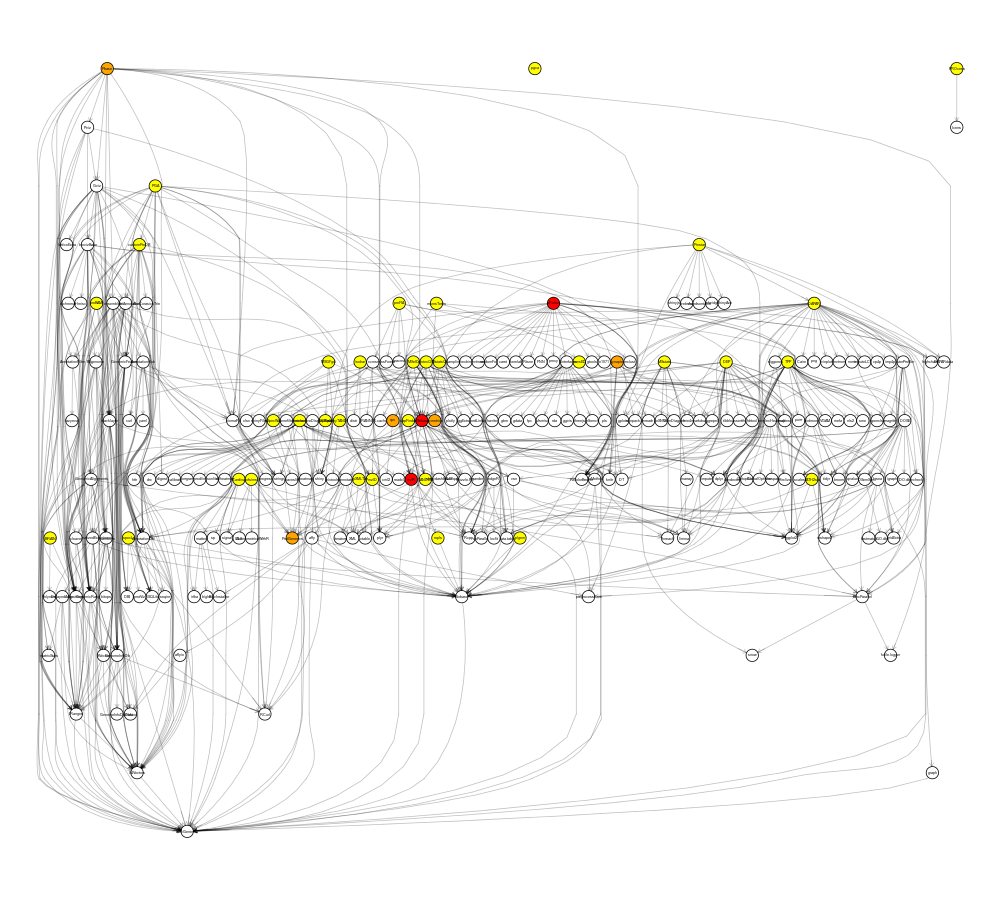
\includegraphics[width=.8\linewidth]{./figs_local/g.png}
    \caption{\textbf{Collaboration between packages}: Dependency graph
      containing 41 MS and proteomics-tagged packages (out of 100+)
      and their dependencies. }
  \end{figure}
\end{frame}

\begin{frame}{\textbf{MSnbase} example}

  \begin{figure}[h]
    \centering
    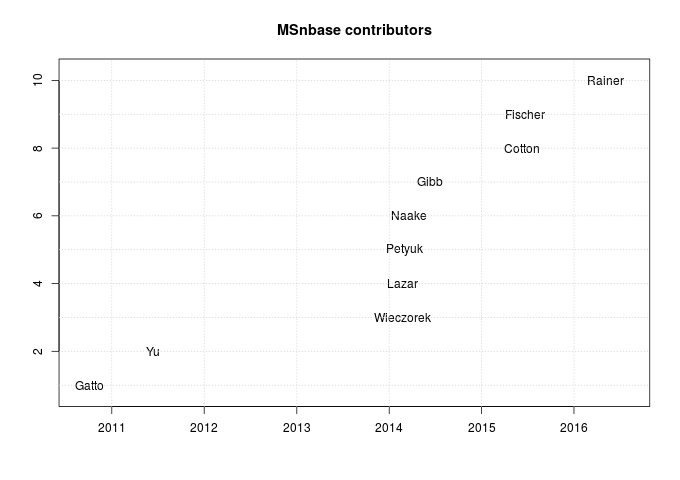
\includegraphics[width=.8\linewidth]{./Figures/msnbase-contributors-2.png}
    \caption{\textbf{Collaboration within packages}: Contributions to the
      \texttt{MSnbase} package (1220 downloads from unique IP
      addresses in January 2018) since its creation, the last one
      leading to \textbf{common proteomics/metabolomics
        infrastructure}. More details:
      \url{https://lgatto.github.io/msnbase-contribs/}}
    \label{fig:msnbase}
  \end{figure}

\end{frame}

\begin{frame}{Open research: open source software}
  \centering
  \begin{figure}
  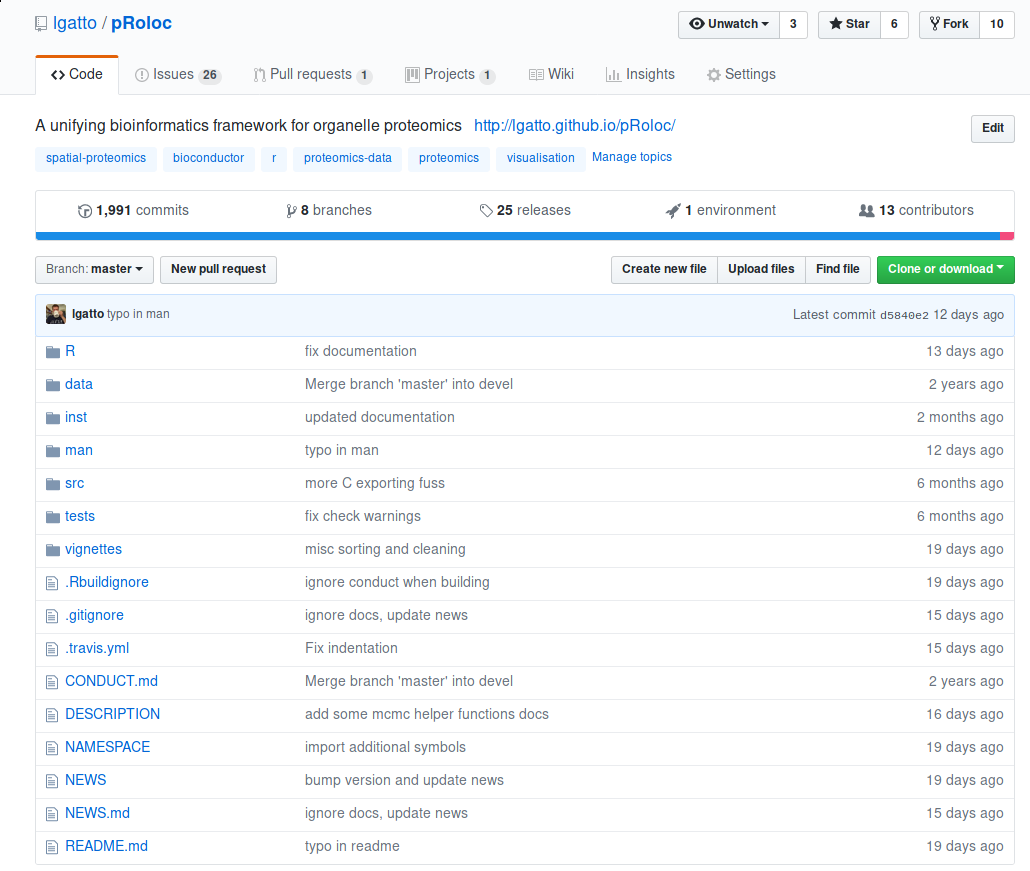
\includegraphics[width=.8\linewidth]{./figs_local/pRoloc_screen.png}
    \caption{Public repository for the \texttt{pRoloc} software
      \url{https://github.com/lgatto/pRoloc}.}
  \end{figure}
\end{frame}

\begin{frame}{Open and reproducible research}
  \centering
  \begin{figure}
    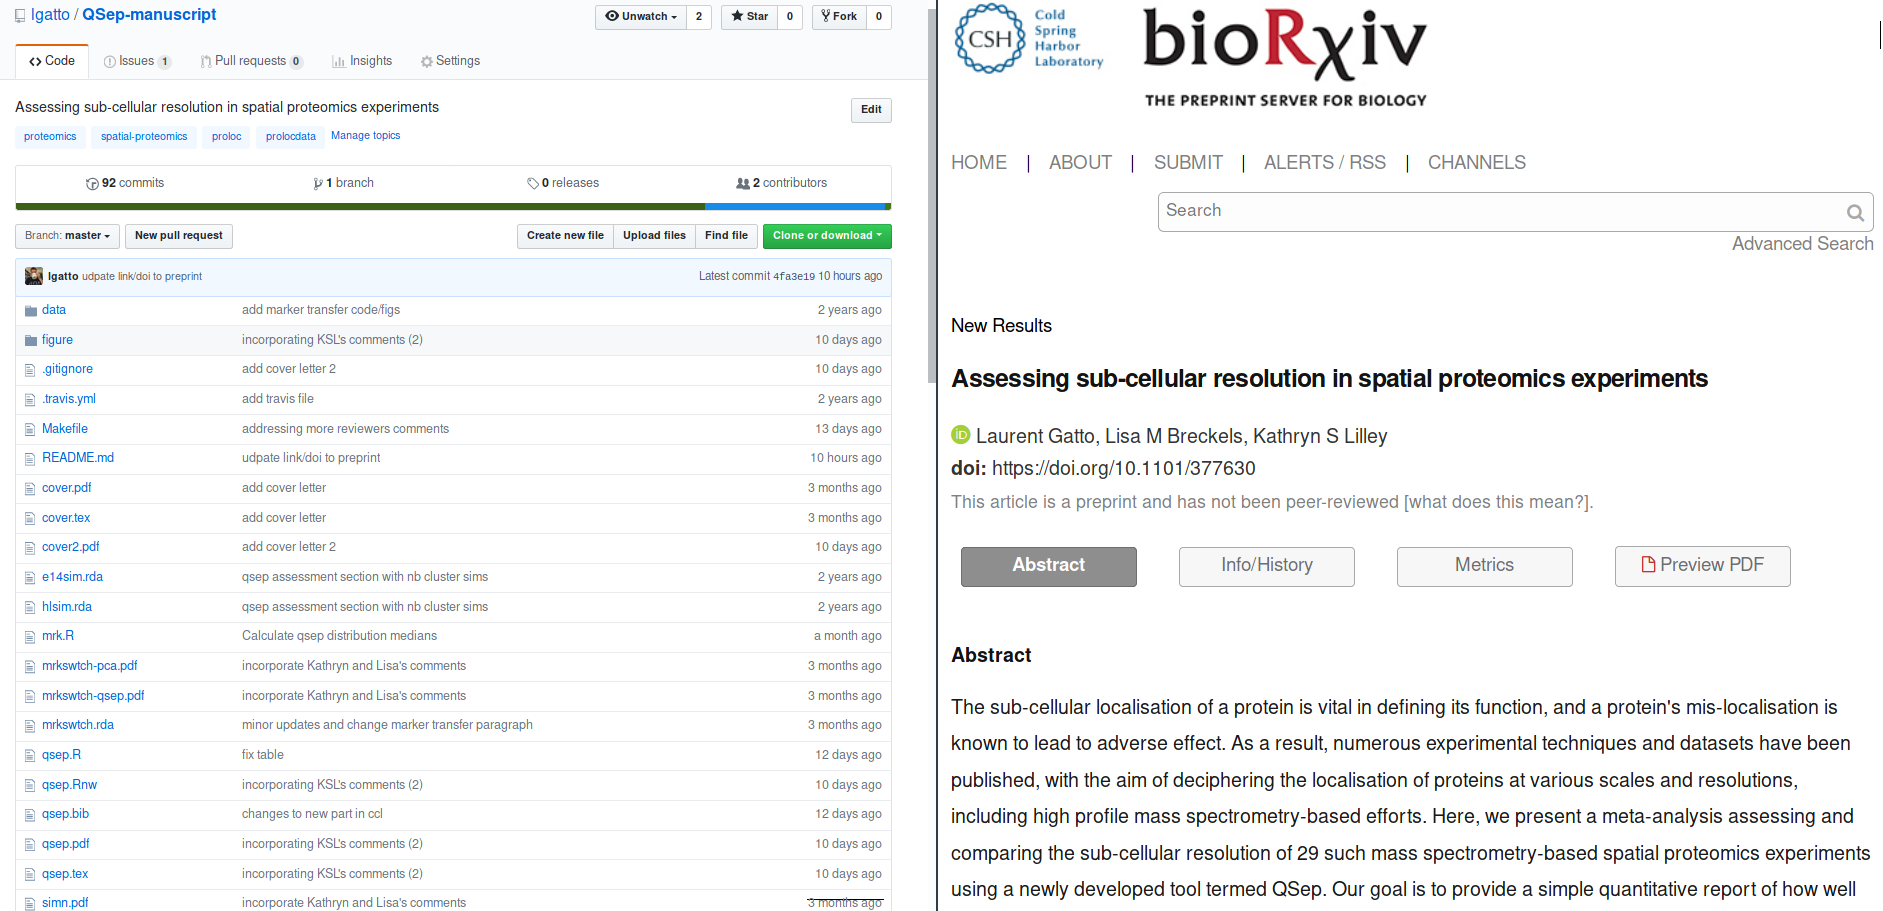
\includegraphics[width=1\linewidth]{./figs_local/qsep_screen.png}
    \caption{\url{https://github.com/lgatto/QSep-manuscript} and
      \url{https://doi.org/10.1101/377630} \citep{Gatto:2018}. In
      press in \textit{Current Opinions in Chemical Biology} now.}
  \end{figure}
\end{frame}

\begin{frame}{}
Working with open and reproducible research in mind doesn't mean
releasing everything prematurely, it means

\begin{itemize}
\item managing research in a way one can find data and results at
  every stage

\item one can reproduce results, re-run/compare them with new data or
  different methods/parameters, and

\item  one can release data (or parts thereof) when/if appropriate.
\end{itemize}
\end{frame}

\begin{frame}{\texttt{MSnSet} data structure}

  \begin{figure}[h]
    \centering
    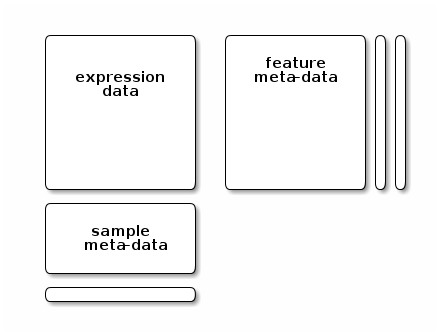
\includegraphics[width=.8\linewidth]{./figs_local/msnset.png}
    \label{fig:msnset}
  \end{figure}

\end{frame}


\begin{frame}[fragile]
\begin{knitrout}
\definecolor{shadecolor}{rgb}{0.969, 0.969, 0.969}\color{fgcolor}\begin{kframe}
\begin{alltt}
\hlkwd{library}\hlstd{(}\hlstr{"pRoloc"}\hlstd{)}
\hlkwd{library}\hlstd{(}\hlstr{"pRolocdata"}\hlstd{)}
\hlkwd{data}\hlstd{(hyperLOPIT2015)}

\hlkwd{setStockcol}\hlstd{(}\hlkwd{paste0}\hlstd{(}\hlkwd{getStockcol}\hlstd{(),} \hlnum{80}\hlstd{))}

\hlkwd{library}\hlstd{(}\hlstr{"magrittr"}\hlstd{)}
\hlkwd{library}\hlstd{(}\hlstr{"dplyr"}\hlstd{)}
\hlkwd{library}\hlstd{(}\hlstr{"ggplot2"}\hlstd{)}
\end{alltt}
\end{kframe}
\end{knitrout}
\end{frame}

\begin{frame}[fragile]
\begin{knitrout}
\definecolor{shadecolor}{rgb}{0.969, 0.969, 0.969}\color{fgcolor}\begin{kframe}
\begin{alltt}
\hlkwd{plot2D}\hlstd{(hyperLOPIT2015,} \hlkwc{fcol} \hlstd{=} \hlkwa{NULL}\hlstd{,}
       \hlkwc{col} \hlstd{=} \hlstr{"#00000025"}\hlstd{,} \hlkwc{pch} \hlstd{=} \hlnum{19}\hlstd{)}
\hlkwd{plot2D}\hlstd{(hyperLOPIT2015,} \hlkwc{method} \hlstd{=} \hlstr{"hexbin"}\hlstd{)}
\hlkwd{plot2D}\hlstd{(hyperLOPIT2015)}

\hlkwd{plot2D}\hlstd{(hyperLOPIT2015,} \hlkwc{fcol} \hlstd{=} \hlstr{"final.assignment"}\hlstd{)}
\hlstd{sz} \hlkwb{<-} \hlkwd{exp}\hlstd{(}\hlkwd{fData}\hlstd{(hyperLOPIT2015)}\hlopt{$}\hlstd{svm.score)} \hlopt{-} \hlnum{1}
\hlkwd{plot2D}\hlstd{(hyperLOPIT2015,} \hlkwc{fcol} \hlstd{=} \hlstr{"final.assignment"}\hlstd{,}
       \hlkwc{cex} \hlstd{= sz)}
\hlkwd{addLegend}\hlstd{(hyperLOPIT2015)}
\end{alltt}
\end{kframe}
\end{knitrout}
\end{frame}

\begin{frame}[fragile]
  \centering
\begin{knitrout}
\definecolor{shadecolor}{rgb}{0.969, 0.969, 0.969}\color{fgcolor}
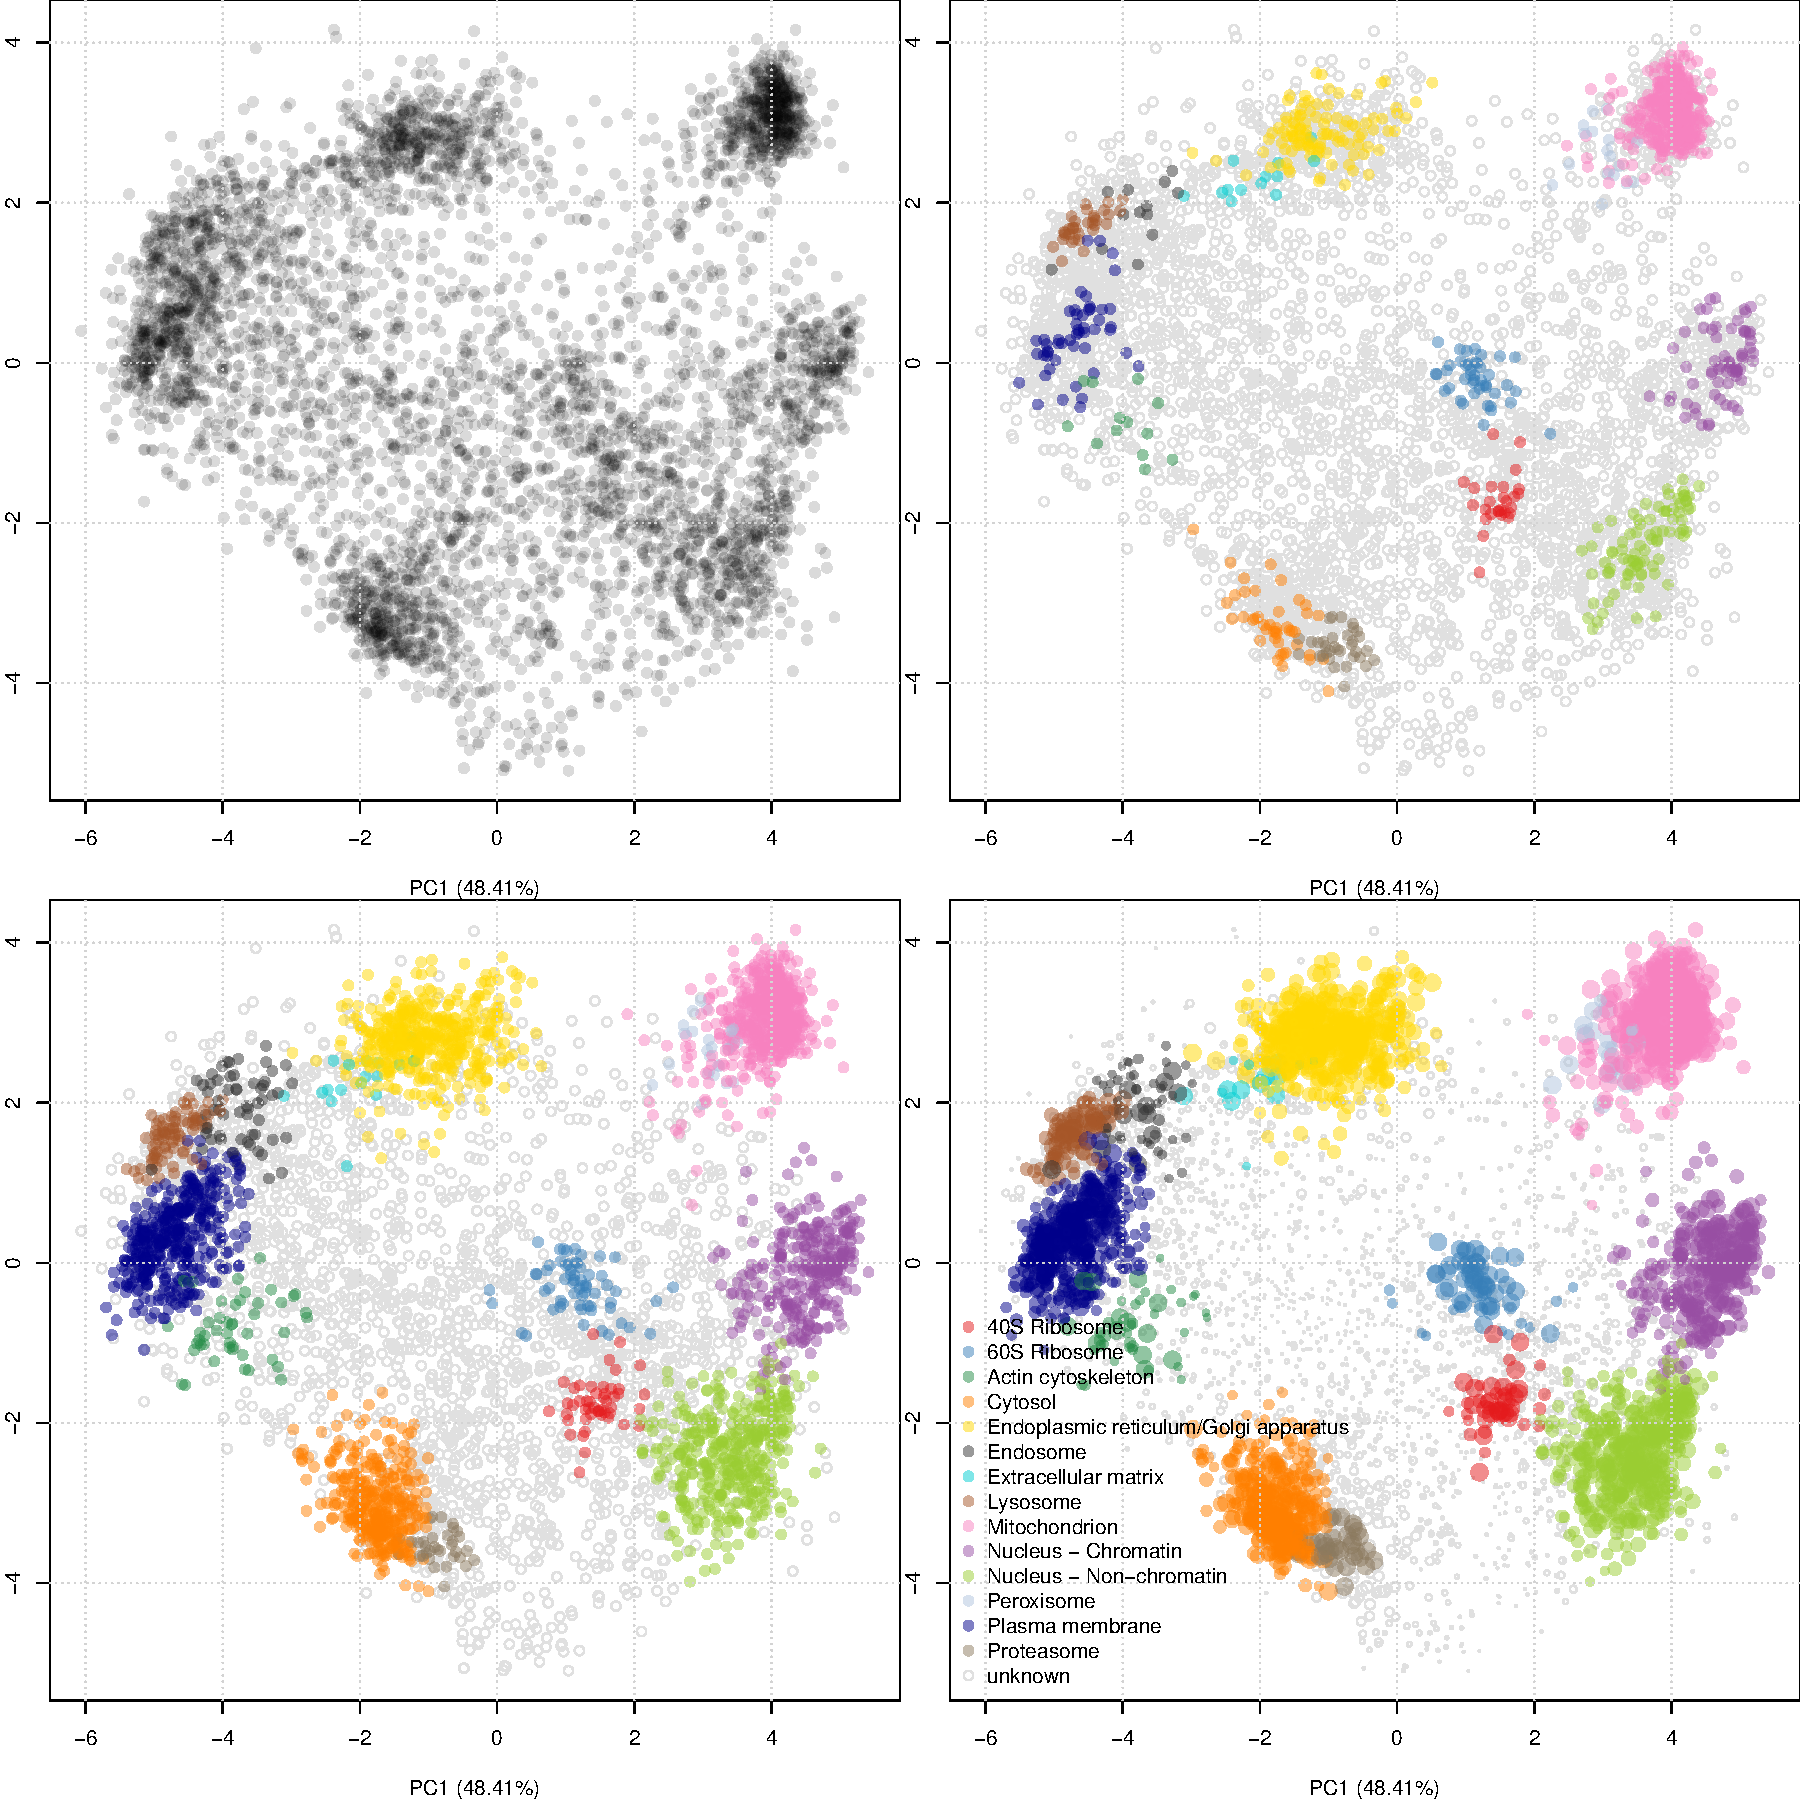
\includegraphics[width=.8\linewidth]{figure/spatprot1eval-1} 

\end{knitrout}
\end{frame}

\begin{frame}[fragile]
  \tiny
\begin{knitrout}
\definecolor{shadecolor}{rgb}{0.969, 0.969, 0.969}\color{fgcolor}\begin{kframe}
\begin{alltt}
\hlkwd{unknownMSnSet}\hlstd{(hyperLOPIT2015)} \hlopt
    \hlstd{fData} \hlopt \hlkwd{select}\hlstd{(final.assignment)} \hlopt \hlstd{table}
\end{alltt}
\begin{verbatim}
## .
##                          40S Ribosome 
##                                    21 
##                          60S Ribosome 
##                                    19 
##                    Actin cytoskeleton 
##                                    33 
##                               Cytosol 
##                                   296 
## Endoplasmic reticulum/Golgi apparatus 
##                                   319 
##                              Endosome 
##                                    47 
##                  Extracellular matrix 
##                                     4 
##                              Lysosome 
##                                    47 
##                         Mitochondrion 
##                                   202 
##                   Nucleus - Chromatin 
##                                   233 
##               Nucleus - Non-chromatin 
##                                   311 
##                            Peroxisome 
##                                     8 
##                       Plasma membrane 
##                                   341 
##                               unknown 
##                                  2225
\end{verbatim}
\end{kframe}
\end{knitrout}
\end{frame}

\begin{frame}[fragile]
    \tiny
\begin{knitrout}
\definecolor{shadecolor}{rgb}{0.969, 0.969, 0.969}\color{fgcolor}\begin{kframe}
\begin{alltt}
\hlkwd{unknownMSnSet}\hlstd{(hyperLOPIT2015)} \hlopt \hlstd{fData} \hlopt
    \hlkwd{select}\hlstd{(final.assignment, svm.score)} \hlopt
    \hlkwd{ggplot}\hlstd{(}\hlkwd{aes}\hlstd{(}\hlkwc{x} \hlstd{= final.assignment,} \hlkwc{y} \hlstd{= svm.score))} \hlopt{+}
    \hlkwd{geom_boxplot}\hlstd{(}\hlkwd{aes}\hlstd{(}\hlkwc{fill} \hlstd{=  final.assignment))}
\end{alltt}
\end{kframe}
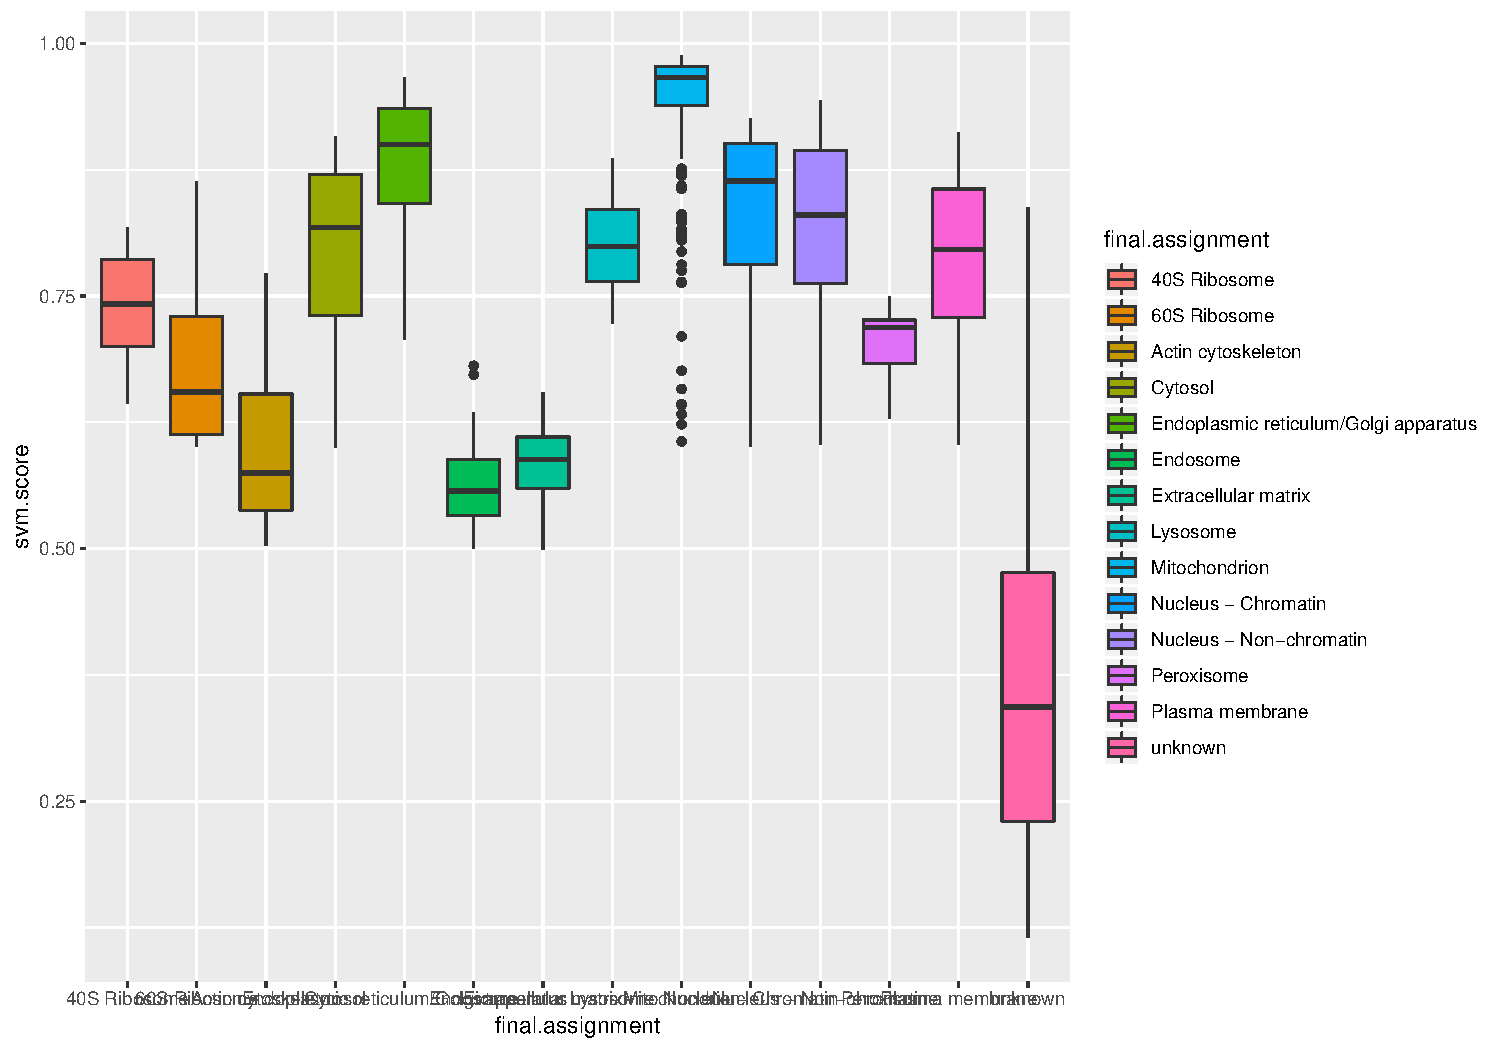
\includegraphics[width=\maxwidth]{figure/spatprot3-1} 

\end{knitrout}
\end{frame}



\begin{frame}[fragile]{Conclusions}
  \begin{itemize}

  \item Protein sub-cellular localisation: technologies (hyperLOPIT)
    and opportunities.

  \item Reliance on computational biology and dedicated software
    (\texttt{pRoloc} \textit{et al.}) to interpret data and acquire
    biological knowledge.

  \item Rigorous computational infrastructure and sound data analysis
    and interpretation is a \textbf{long term investment}.

  \end{itemize}

\end{frame}


\begin{frame}[allowframebreaks]{References}
  \tiny
  \bibliographystyle{plainnat}
  \bibliography{spatial_proteomics,bib2}
\end{frame}


\begin{frame}
  \begin{block}{Acknowledgements}
    \begin{itemize}
    \item \textbf{Mr Oliver Crook} and \textbf{Dr Lisa Breckels},
      Computational Proteomics Unit, Cambridge (machine learning,
      algorithms, software).
    \item \textbf{Dr Sebastian Gibb} and \textbf{Dr Johannes Rainer}
      (software).
    \item \textbf{Prof Kathryn Lilley} \textit{et al.}, Cambridge
      Centre of Proteomics and \textbf{Dr Claire Mulvey}, Cancer
      Research UK Cambridge Institute (spatial proteomics)
    \item \textbf{Funding}: BBSRC, Wellcome Trust
    \end{itemize}
  \end{block}



  \begin{center}
    \textbf{Thank you for your attention}
  \end{center}

\end{frame}

%% \include{add}

\end{document}
